\section{Design}
\subsection{Socket Listener}

\begin{figure}[H]
\centering
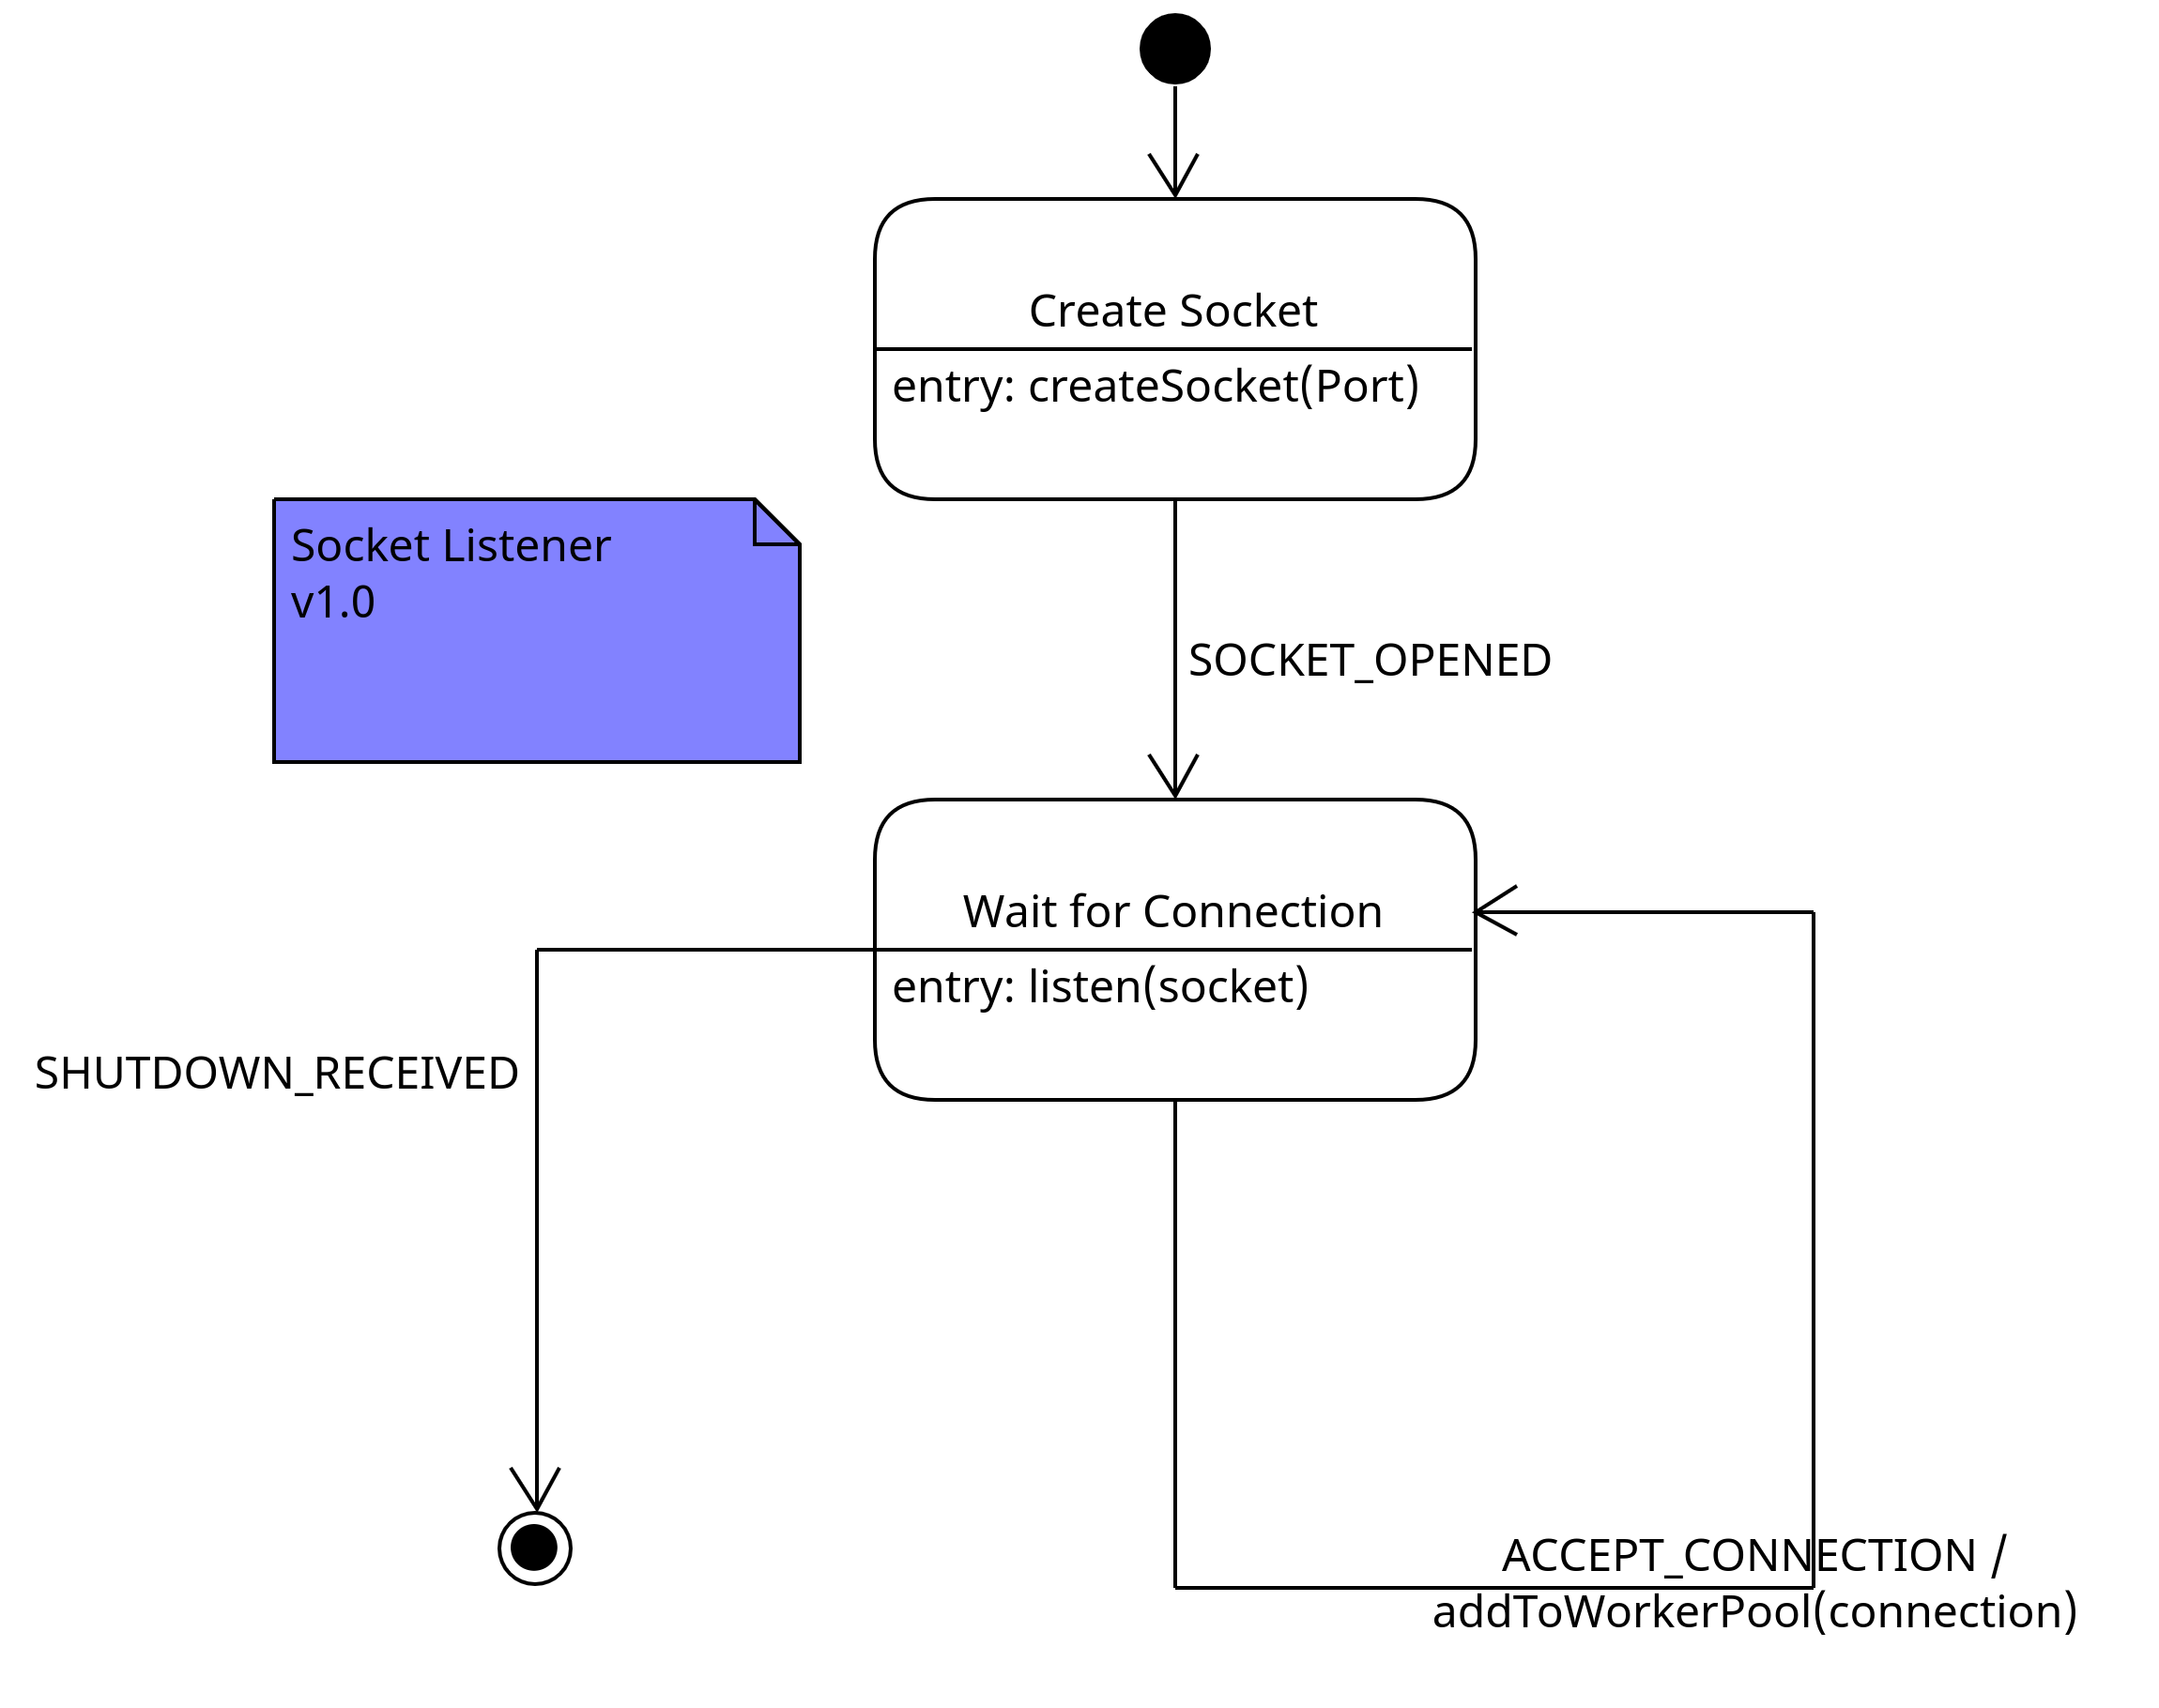
\includegraphics[width=0.8\textwidth]{images/socketlistener.png}
\caption{Socket Listener}
\label{fig:SocketListener}
\end{figure}

Um die Kommunikation mit anderen Teilnehmern des Netwerkes zu ermöglichen, wird ein Socket Listener benötigt. 
Dieser lauscht auf einem Port und empfängt Verbindungsanfragen von anderen Teilnehmern.
Diese werden dann in den Thread Pool übergeben, der die Verbindung dann in einem eigenen Thread behandelt.
Der Socket Listener wird in einem eigenen Thread ausgeführt, damit die Anwendung nicht blockiert wird.

\subsection{Socket Handler}

\begin{figure}[H]
\centering
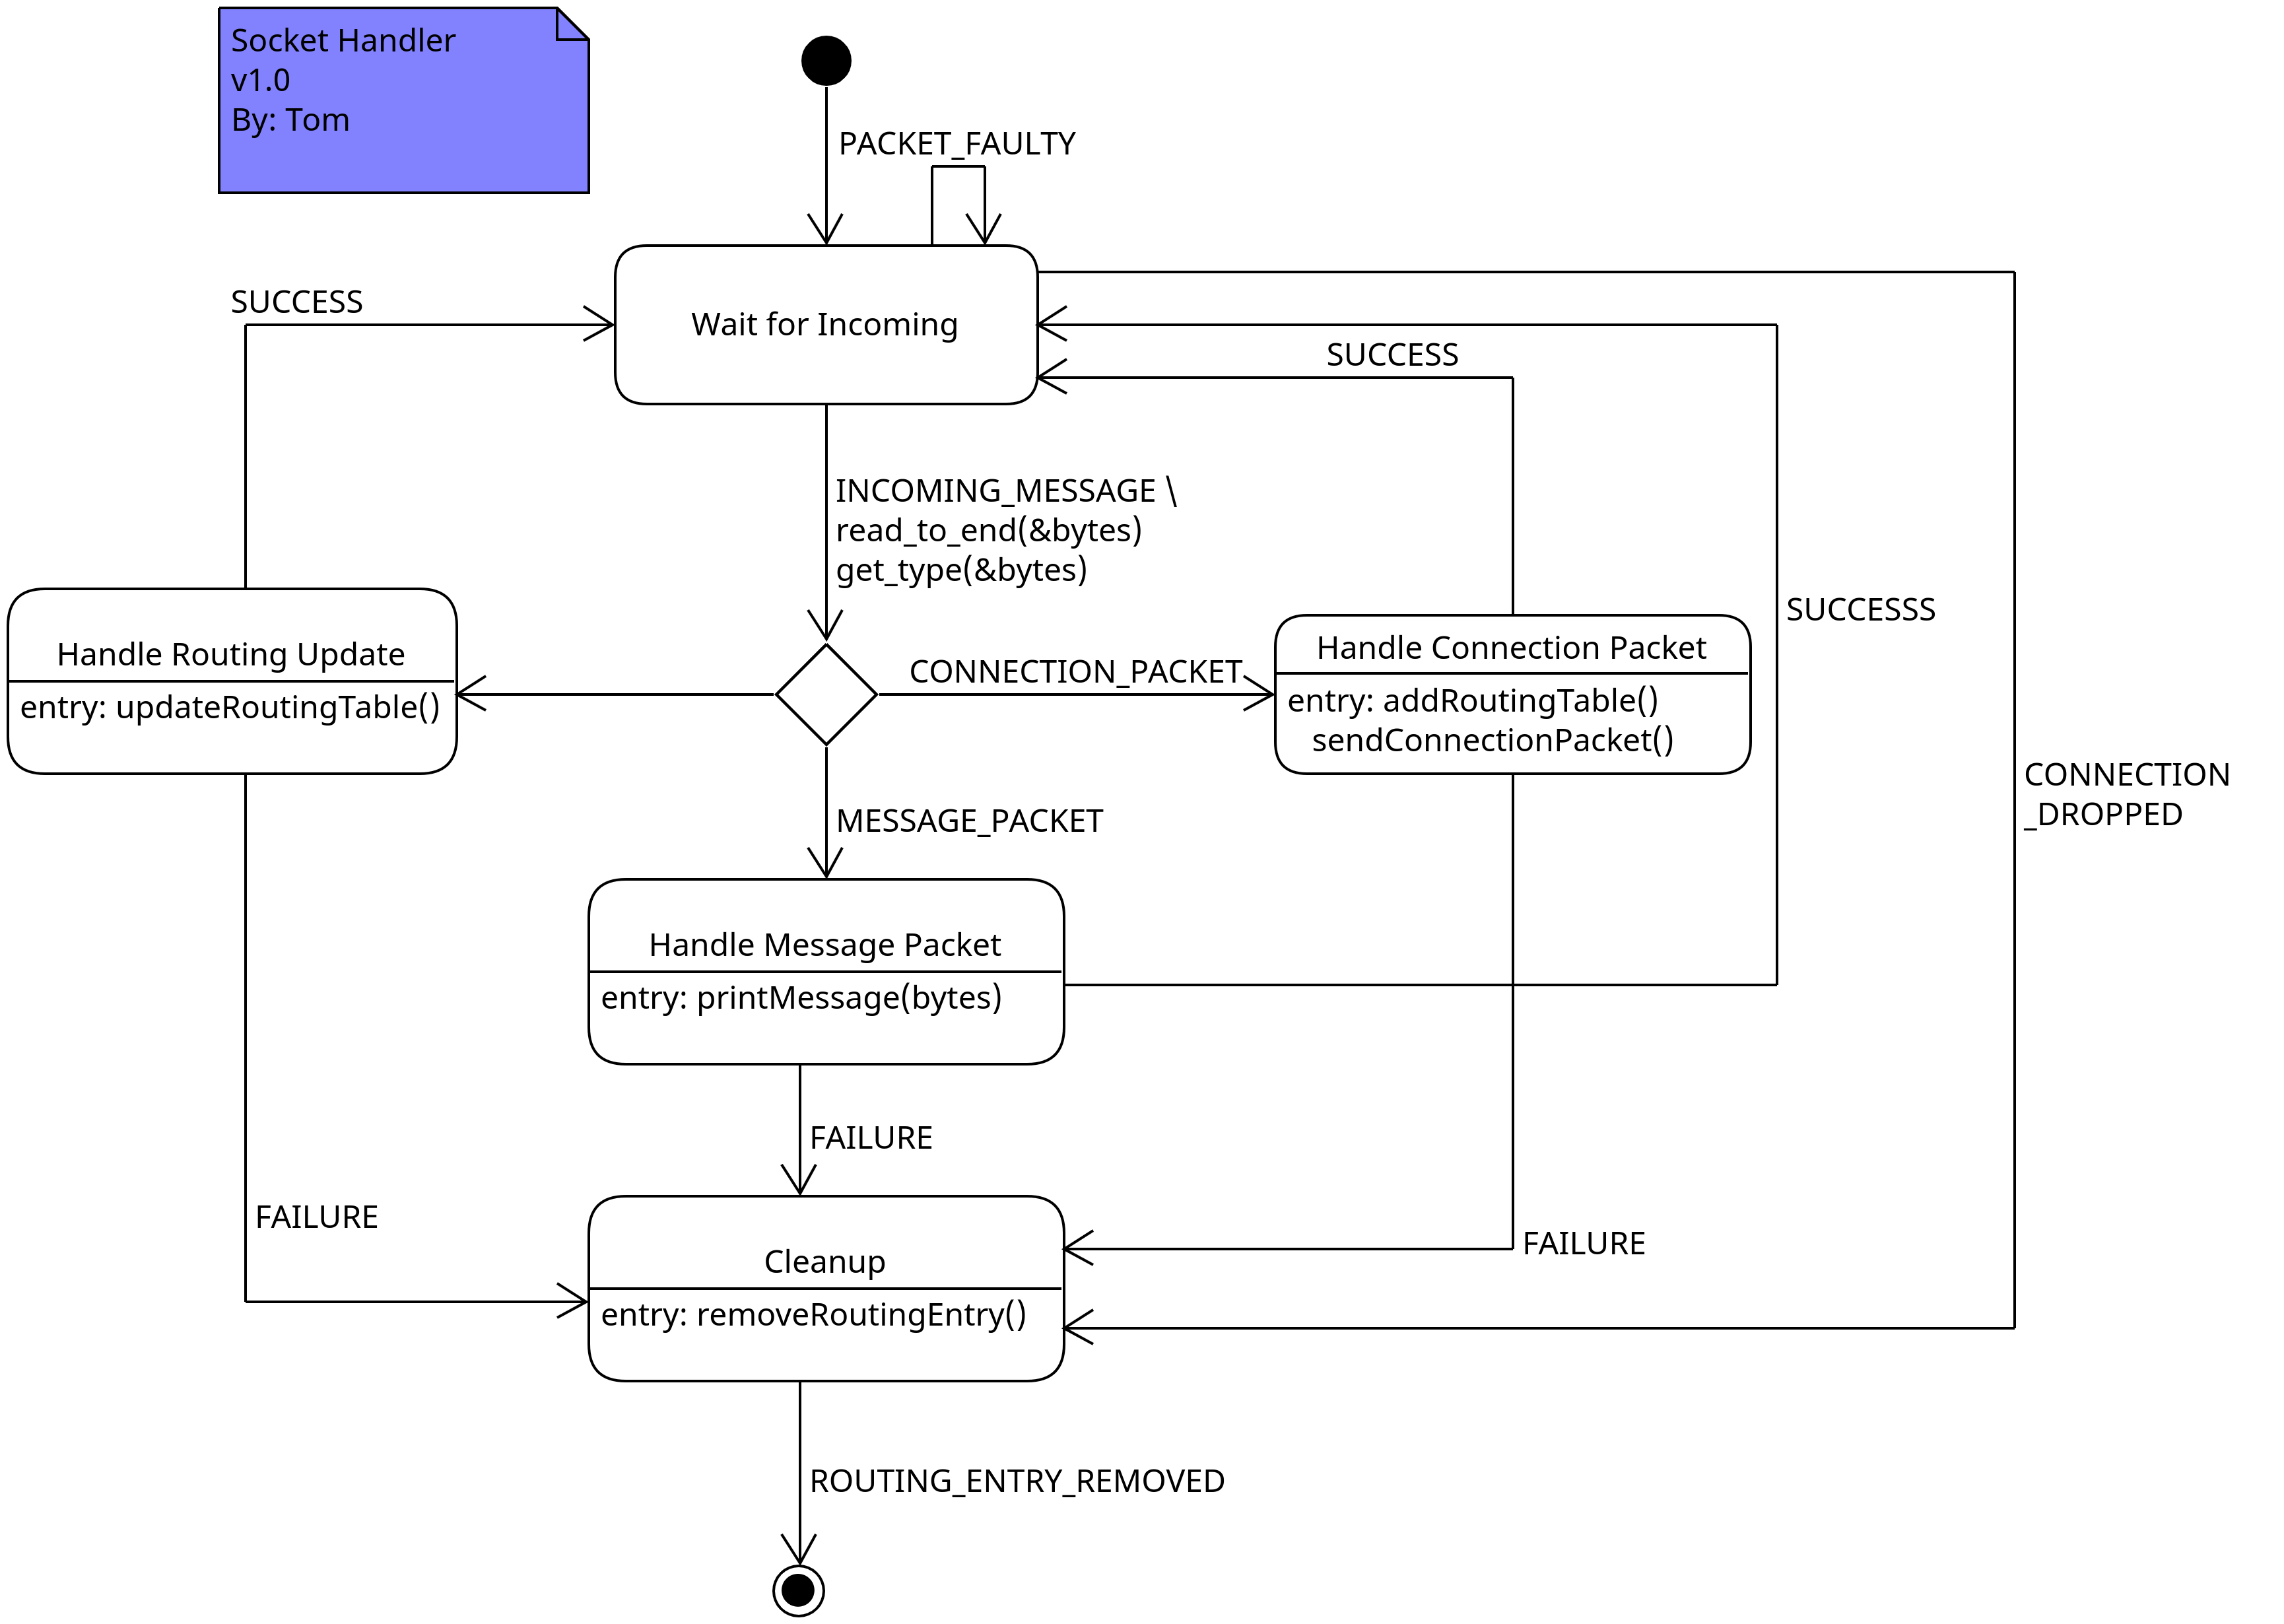
\includegraphics[width=0.8\textwidth]{images/sockethandler.png}
\caption{Socket Handler}
\label{fig:SocketHandler}
\end{figure}

Der Socket Handler ist für die Kommunikation mit einem anderen Teilnehmer zuständig, spezifisch für der Empfangen von Nachrichten.
Er wird vom Socket Listener in einem eigenen Thread innerhalb des Thread Pools ausgeführt. 
Dabei wird unterschieden um welchen Typen es sich bei der Nachricht handelt und das Paket jeweils verifiziert mit CRC32.
Bei einem Fehler wird das Paket verworfen und der Socket Handler beendet,
 wobei vorher immer die Verbindung aus der Routing Tabelle entfernt wird.

 \subsection{TUI}

\begin{figure}[H]
\centering
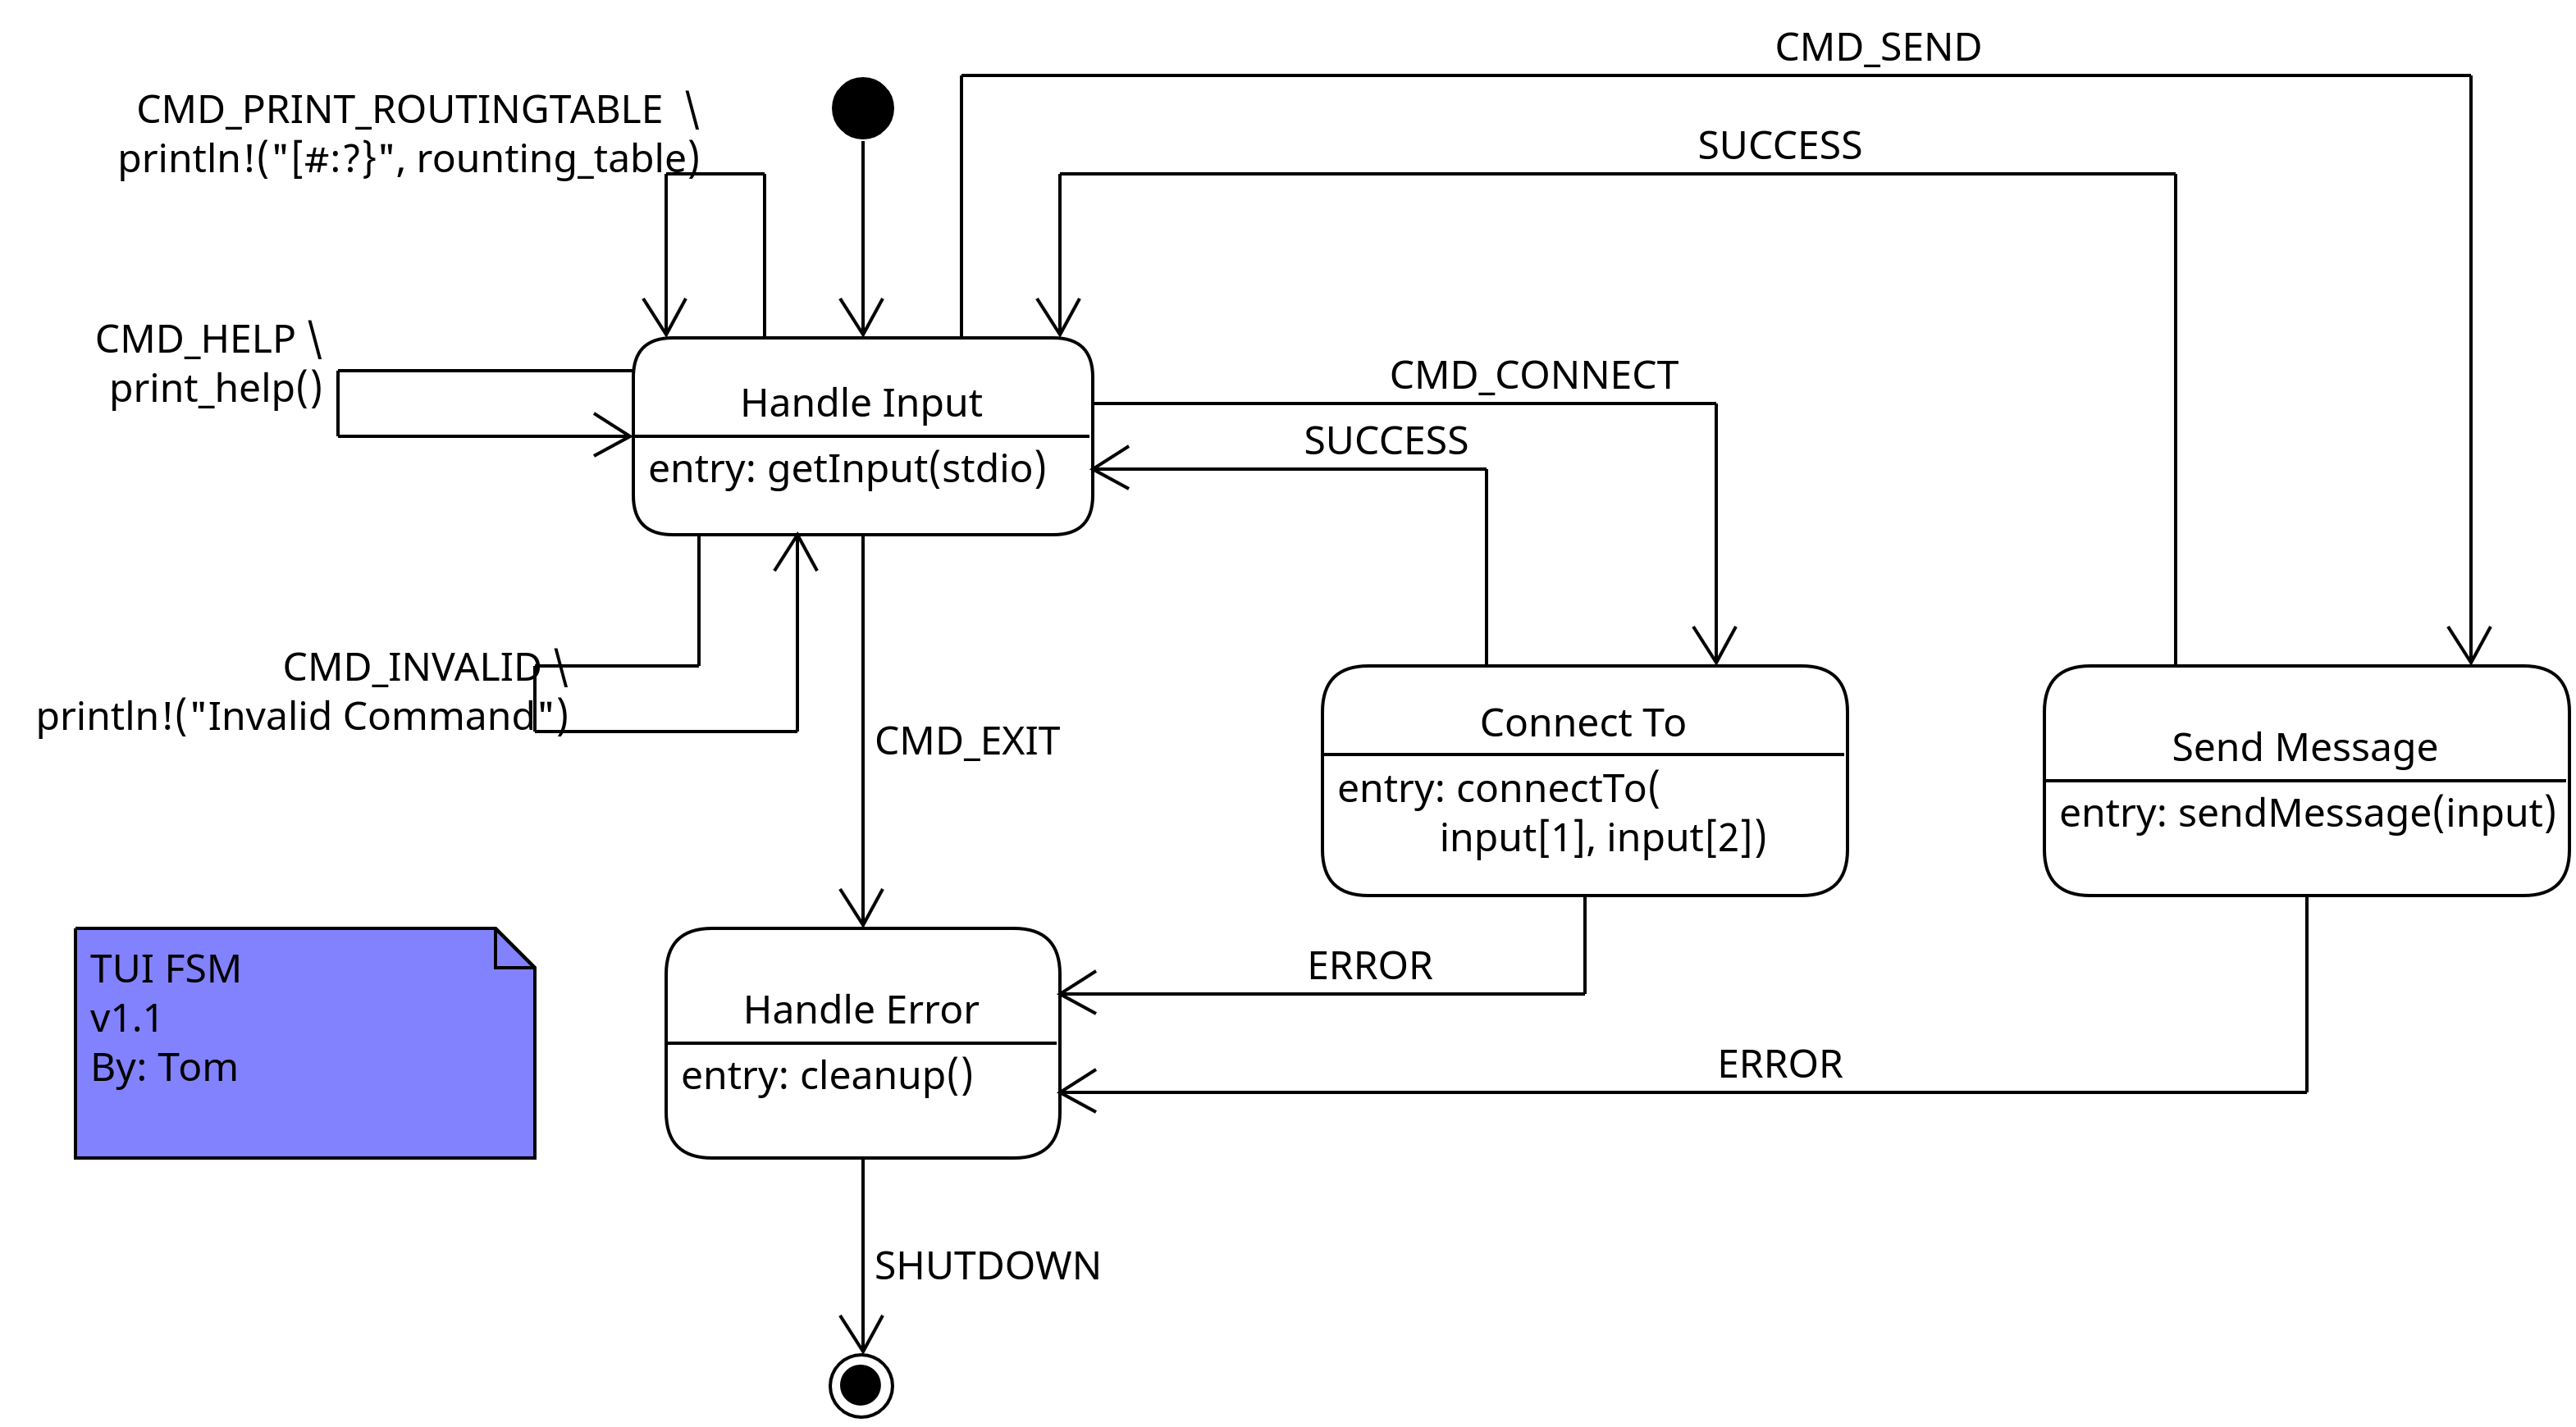
\includegraphics[width=0.8\textwidth]{images/tui.png}
\caption{TUI}
\label{fig:TUI}
\end{figure}

Die TUI ist für die Interaktion mit dem Benutzer zuständig. Sie nimmt sich jeweils eine Linieneingabe und verarbeitet diese.
Dabei wird das erste Wort als Befehl interpretiert und die restlichen Wörter als Argumente.
Die TUI ist in einem eigenen Thread, damit die Anwendung nicht blockiert wird.
Bei einem Fehler durch falsche Eingabe wird eine Fehlermeldung ausgegeben und die TUI wartet auf die nächste Eingabe.
Bei einem kritischen Fehler wird die Anwendung beendet, dies kann auch durch den Befehl \textit{exit} geschehen.
Die Ausgabe aller Befehle erfolgt durch den Befehl \textit{help}.

\newpage
\subsection{Routingtabelle}
Die Routingtabelle speichert Informationen zu allen verfügbaren Clienten:
\\
\begin{center}
\begin{tabular}{|c|c|c|c|c|c|c|}
\hline
info\_source & destination & ip & port & hops & ttl & dont\_expire
\\ \hline
\end{tabular}
\end{center}
\begin{itemize}
    \item \textbf{info\_source:} Die Quelle eines Eintrags und damit der nächste Hop für Pakete auf der Route zur destination.
    \item \textbf{destination:} 
    \item \textbf{ip:} Die IP Adresse der destination wenn diese verbunden ist oder des nächsten Hops.  
    \item \textbf{port:} Der Port der destination wenn diese verbunden ist oder des nächsten Hops.
    \item \textbf{hops:} die Länge der Route zur destination in Clients an/über die Pakete gesendet werden müssen.
    \item \textbf{ttl:} Die Lebenszeit eines Eintrags beginnend mit 30. 
    \item \textbf{dont\_expire:} Wenn dieser boolean true ist läuft der Eintrag nicht ab, wird also nicht aus der Routingtabelle entfernt.
\end{itemize}
Einmal die Sekunde werden alle Einträge mit einer TTL niedriger als 1 und ohne dont\_expire aus der Routingtabelle entfernt und die TTL aller Einträge um 1 reduziert.

\noindent Neue Einträge werden der Routingtabelle bei neuen Verbindungen oder bei Routingupdates hinzugefügt oder aktualisiert und die Routingtabelle so möglichst aktuell gehalten.

\noindent Der Client sendet Routingupdates alle 15 Sekunden an verbundene Clienten und bekommt in einem 15 Sekunden Takt von verbundenen Clienten Routingupdates.

\textbf{FSMs für diese beiden Loops? Die sind kinda banal.}